\documentclass[tikz,border=8pt]{standalone}
\usepackage{amsmath}
\usetikzlibrary{arrows.meta,positioning,fit}

\begin{document}
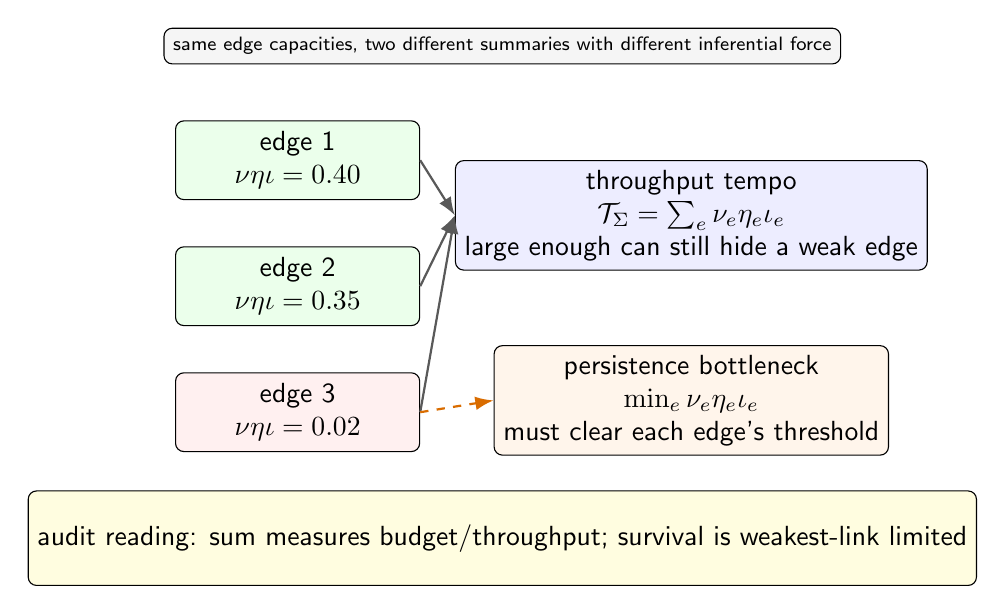
\begin{tikzpicture}[
  font=\sffamily,
  edgebox/.style={draw, rounded corners=3pt, align=center, minimum width=31mm, minimum height=10mm, fill=white},
  box/.style={draw, rounded corners=3pt, align=center, minimum width=44mm, minimum height=12mm, fill=white},
  note/.style={align=center, font=\sffamily\scriptsize},
  arrow/.style={-Latex, thick, draw=black!65},
  warn/.style={-Latex, thick, dashed, draw=orange!85!black}
]

\node[edgebox, fill=green!8] (e1) at (0,1.6) {edge 1\\$\nu\eta\iota=0.40$};
\node[edgebox, fill=green!8] (e2) at (0,0) {edge 2\\$\nu\eta\iota=0.35$};
\node[edgebox, fill=red!6] (e3) at (0,-1.6) {edge 3\\$\nu\eta\iota=0.02$};

\node[box, fill=blue!7] (sum) at (5,0.9)
  {throughput tempo\\$\mathcal T_\Sigma=\sum_e \nu_e\eta_e\iota_e$\\large enough can still hide a weak edge};
\node[box, fill=orange!8] (min) at (5,-1.45)
  {persistence bottleneck\\$\min_e \nu_e\eta_e\iota_e$\\must clear each edge's threshold};

\draw[arrow] (e1.east) -- (sum.west);
\draw[arrow] (e2.east) -- (sum.west);
\draw[arrow] (e3.east) -- (sum.west);
\draw[warn] (e3.east) -- (min.west);

\node[box, fill=yellow!12, minimum width=88mm] at (2.6,-3.2)
  {audit reading: sum measures budget/throughput; survival is weakest-link limited};

\node[note, fill=gray!8, draw, rounded corners=3pt, minimum width=82mm] at (2.6,3.05)
  {same edge capacities, two different summaries with different inferential force};

\end{tikzpicture}
\end{document}
